\chapter{Reti di flusso}\label{app:flownet}

    Formalmente una \textit{rete di flusso} è definita come un grafo orientato $G = (V, E)$ tale che
    \begin{itemize}
        \item Ad ogni arco $(u,v) \in E$ e associato un valore non negativo, $c(u, v) \ge 0$, detto \textit{capacità} dell'arco. Se il nodo $(u, v)$ non è presente in $E$ allora assumiamo che l’arco $(u, v)$ abbia capacità nulla, cioè $c(u, v) = 0$.
        \item Nella rete di flusso ci sono due vertici speciali: il vertice \textit{sorgente} (o \textit{source}), indicato con il simbolo $s$, ed il vertice \textit{pozzo} (o \textit{sink}), indicato con il simbolo $t$.
        \item Ogni vertice giace su qualche cammino dalla sorgente al pozzo. Il grafo è quindi connesso e pertanto vale $|E| \ge |V | - 1$.
    \end{itemize}

    La Figura \ref{fig:flownet} mostra un esempio di rete di flusso. La sorgente ed il pozzo sono rappresentati, rispettivamente, dai simboli $s$ e $t$. Ad ogni arco $(u, v) \in E$ è associato il valore $c(u, v)$.
    
    \begin{figure}[h]
        \centering
        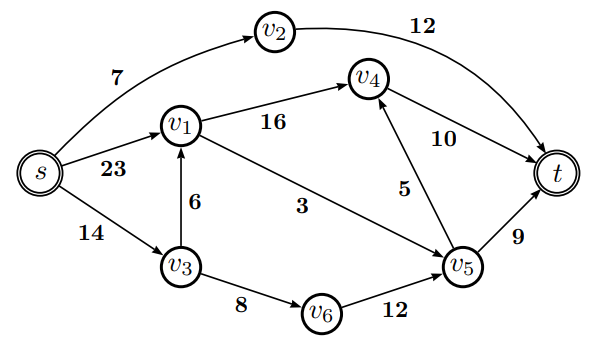
\includegraphics[width=0.6\linewidth]{images/flownet.png}
        \caption{Rete di flusso}
        \label{fig:flownet}
    \end{figure}


    \section{Flusso}

        Per \textit{flusso} in una rete si intende una funzione $x : E \rightarrow \mathbb{R}$ che rispetta i vincoli di capacità del grafo ovvero:
        \begin{equation}
            0 \le x_{ij} \le c(i,j) \quad \forall (i,j) \in E
        \end{equation}

        Con il termine \textit{divergenza} di un nodo $i$ si intende la differenza tra il flusso uscente e quello entrante ovvero, dato un nodo $v \in V$ e un flusso $x$ in $G$:
        \begin{equation}
            \Delta_x(v) = \sum_{\mathclap{\substack{j \in V \\ (v,j) \in E}}}x_{vj} - \sum_{\mathclap{\substack{i \in V \\ (i,v) \in E}}}x_{iv}
        \end{equation}

        Si dice che il flusso $x$ è conservato nel nodo $v$ (o che il flusso $x$ soddisfa i vincoli di conservazione del flusso) se $\Delta_x(v) = 0$. Un flusso che è conservato per ogni nodo è detto \textit{circolazione}. Una \textit{circolazione} può essere vista come uno scambio di beni in cui nulla viene mai creato o distrutto, ma è semplicemente passato da un nodo all'altro.

        Se un flusso non è una circolazione, assumendo $S:=\{v : \Delta_x(v) > 0 \}$ e $T:=\{v : \Delta_x(v) < 0 \}$, possiamo interpretare il flusso come uno spostamento di beni in quantità $\phi = \sum_{v \in S} \Delta_x(v)$ dai nodi in $S$ a quelli in $T$. Infatti, tutto il flusso uscente da $S$ entrerà nei nodi in $T$.

        Se consideriamo $s$ (source) e $t$ (sink) due nodi distinti in $V$, ogni flusso che è conservato in ogni nodo $v \neq s,t$ è chiamato \textit{flusso s-t} e il suo valore è definito come:
        \begin{equation}
            \phi_x = \Delta_x(s)
        \end{equation}

        Il problema del trovare il flusso s-t con valore massimo (dati $s$ e $t$) all'interno di una rete è chiamato \textit{problema del massimo flusso} \cite{Lancia2022}.
        
    \section{Rete residua}
        Sia $f$ un flusso in una rete (G, c), e si consideri una coppia di vertici $u, v \in V$ . La quantità di flusso che possiamo inviare da $u$ a $v$ prima di superare la capacità $c(u, v)$ è la \textit{capacità residua} di $(u, v)$, ed è data da 
        \begin{equation}
            c_f (u, v) = c(u, v) - f(u, v)
        \end{equation}

        Data una rete di flusso $(G, c)$ ed un flusso $f$, la rete residua di $G$ indotta da $f$ è $G_f = (V, E_f )$, dove
        \begin{equation}
            E_f = \{(u, v) \in V \times V : c_f(u, v) > 0\}
        \end{equation}
        
        Ogni arco della rete, chiamato \textit{arco residuo}, può ammettere un flusso strettamente positivo.
        Un arco $(u, v)$ può essere un arco residuo in $E_f$ , anche se esso non fosse un arco in $E$, ma purché $(v, u) \in E$. Ciò implica che non sempre vale la relazione $E_f \subseteq E$. Però si ha sempre
        \begin{equation}
            |E_f| \le 2 \cdot |E|
        \end{equation}
        
        Si osservi che la rete residua $G_f$ è essa stessa una rete di flusso avente capacità definita dalla funzione $c_f$.
    